\documentclass{beamer}
\usepackage[utf8]{inputenc}
\usepackage[italian]{babel}
\usepackage{colortbl}% for color in text
\usepackage{xcolor}% for color in text
\usepackage{siunitx} % for numbers units
\usepackage{booktabs}% for tables
\usepackage{pgfplots}% for plots
\usepackage{multirow}% for tables
\usepackage{array}
\pgfplotsset{label style={font=\footnotesize},tick label style={font=\footnotesize}}
\usetheme{Boadilla} 
\setbeamercolor{section in head/foot}{fg=black, bg=white}
\title{Sintesi e caratterizzazione di politiofeni chirali.}
\date{15 ottobre 2013}
\institute{Dipartimento di Chimica e Chimica Industriale -- Università di Pisa}
\hypersetup{pdfauthor={Ilario Gelmetti},pdfsubject={},pdfkeywords={},pdftitle={}}
\newcommand{\tallcell}[2][c]{\begin{tabular}[#1]{@{}c@{}}#2\end{tabular}}
\newcommand{\tallcellerre}[2][c]{\begin{tabular}[#1]{@{}r@{}}#2\end{tabular}}
\newcommand{\tallcellelle}[2][c]{\begin{tabular}[#1]{@{}l@{}}#2\end{tabular}}
\setbeamertemplate{navigation symbols}{}
\logo{\includegraphics[width=0.1\paperwidth]{img/unipi-logo_con_testo-small.png}}

\makeatletter
\setbeamertemplate{footline}
{
  \leavevmode%
  \hbox{%
  \begin{beamercolorbox}[wd=.20\paperwidth,ht=2.25ex,dp=1ex,center]{section in head/foot}%
    \usebeamerfont{author in head/foot}Ilario Gelmetti
  \end{beamercolorbox}%
  \begin{beamercolorbox}[wd=.55\paperwidth,ht=2.25ex,dp=1ex,center]{section in head/foot}%
    \usebeamerfont{title in head/foot}\insertsection
%   \end{beamercolorbox}%
%   \begin{beamercolorbox}[wd=.05\paperwidth,ht=2.25ex,dp=1ex,center]{section in head/foot}%
  \hfill $>$ \hfill
%   \end{beamercolorbox}%
%   \begin{beamercolorbox}[wd=.20\paperwidth,ht=2.25ex,dp=1ex,center]{section in head/foot}%
    \usebeamerfont{title in head/foot}\insertsubsection
  \end{beamercolorbox}%
  \begin{beamercolorbox}[wd=.25\paperwidth,ht=2.25ex,dp=1ex,right]{section in head/foot}%
    \usebeamerfont{date in head/foot}\insertshortdate{}\hspace*{2em}
    \insertframenumber{} / \inserttotalframenumber\hspace*{2ex} 
  \end{beamercolorbox}}%
  \vskip0pt%
}
\makeatother

\newcommand{\backupbegin}{
  \newcounter{framenumberappendix}
  \setcounter{framenumberappendix}{\value{framenumber}}
}
\newcommand{\backupend}{
  \addtocounter{framenumberappendix}{-\value{framenumber}}
  \addtocounter{framenumber}{\value{framenumberappendix}} 
}

\begin{document}

\author[Ilario Gelmetti]{\begin{tabular}{r@{ }l} 
{\small Autore:} & Ilario Gelmetti \\
&\texttt{\tiny ilario.gelmetti@sns.it, iochesonome@gmail.com}  \\[3ex] 
{\small Relatori:} & Silvia Destri\\
& Lorenzo Di Bari
\end{tabular}}

\section{Tesi magistrale}
\subsection{Chimica organica}
\begin{frame}
\titlepage
\begin{center}
\includegraphics[width=0.12\textwidth]{img/cc-by-sa.pdf}
\end{center}
\end{frame}
%X--%X--%X--%X--%X--%X--%X--%X--%X--%X--%X--%X--%X--%X--%X--%X--%X--%X--%X--%X--%X--%X--%X--%X--%X--%X--%X--%X--%X--%X--%X--
%X--%X--%X--%X--%X--%X--%X--%X--%X--%X--%X--%X--%X--%X--%X--%X--%X--%X--%X--%X--%X--%X--%X--%X--%X--%X--%X--%X--%X--%X--%X--
\section{Il fotovoltaico \& fotovoltaico organico}
\subsection{Ambito}
\begin{frame}% ============== ambito ============== 
\frametitle{Qual è l'ambito del progetto di tesi?}

PRIN 2009 ``\textbf{Materiali innovativi per fotovoltaico organico e ibrido}''
\pause
\vfill
\begin{tabular}{rl}
\textbf{ISMAC-CNR, Milano}: & \tallcellelle{\textbf{Sintesi e caratterizzazione}\\ molecolare e strutturale.}\\[0.5ex]  \\

\textbf{DCCI-Università di Pisa}: & \tallcellelle{Caratterizzazione di \textbf{dicroismo}\\ \textbf{circolare} elettronico.}\\[0.5ex]  \\

\multicolumn{2}{c}{\onslide<3->{Collaborazioni con:}}\\[0.5ex]  \\

\onslide<3->{
ICTP-CNR, Catania:} & \onslide<3->{\tallcellelle{Caratterizzazione MALDI-TOF MS\\ e SEC/MALDI-TOF MS.}}\\[0.5ex]  \\

\onslide<3->{\tallcellerre{CHOSE-Università\\ di Roma Tor Vergata:}} & \onslide<3->{Test dei materiali in cella solare.}\\

\end{tabular}
\end{frame}
%X--%X--%X--%X--%X--%X--%X--%X--%X--%X--%X--%X--%X--%X--%X--%X--%X--%X--%X--%X--%X--%X--%X--%X--%X--%X--%X--%X--%X--%X--%X--
%X--%X--%X--%X--%X--%X--%X--%X--%X--%X--%X--%X--%X--%X--%X--%X--%X--%X--%X--%X--%X--%X--%X--%X--%X--%X--%X--%X--%X--%X--%X--
\subsection{Cos'è?}
\begin{frame}% ============== cos'è ============== 
\frametitle{Cos'è il fotovoltaico \emph{organico}?}
Nelle celle solari \textbf{tradizionali} inorganiche si usa \\\textbf{silicio drogato \textit{n}} (con elettroni liberi) e \textbf{silicio drogato \textit{p}} (con lacune libere).
\vfill \pause
\begin{tabular}{lc}
\tallcell{Nelle celle solari \emph{organiche} si usa: \medskip \\

1. un materiale \textbf{elettron donatore} \\(materiale \textit{p}, ad es.\ un \textbf{polimero coniugato}, \\ assorbe i fotoni),} &\begin{minipage}{0.3\textwidth}\begin{figure}\centering\includegraphics[width=1\textwidth]{img/politiofene-red.pdf}\end{figure}\end{minipage} \\
\onslide<3->{\tallcell{2. un diverso materiale elettron \textbf{accettore}\\ (materiale \textit{n}, ad es.\ derivati del \textbf{fullerene}).}} & \onslide<3->{\begin{minipage}{0.25\textwidth}\begin{figure}\centering\includegraphics[width=1\textwidth]{img/PCBM-mezzo-colorato.pdf}\end{figure}\end{minipage}} \\
\end{tabular}
\end{frame}
%X--%X--%X--%X--%X--%X--%X--%X--%X--%X--%X--%X--%X--%X--%X--%X--%X--%X--%X--%X--%X--%X--%X--%X--%X--%X--%X--%X--%X--%X--%X--
%X--%X--%X--%X--%X--%X--%X--%X--%X--%X--%X--%X--%X--%X--%X--%X--%X--%X--%X--%X--%X--%X--%X--%X--%X--%X--%X--%X--%X--%X--%X--
\subsection{Vantaggi}
\begin{frame}% ============== vantaggi ============== 
\frametitle{Quali i vantaggi del fotovoltaico organico?}
La purificazione del silicio è un processo costoso e resterà costoso.
\vfill
I moduli fotovoltaici organici possono essere \\ più \textbf{economici}, più \textbf{leggeri} e \textbf{flessibili}.
\vfill\pause
{\color{red} \textbf{Ma:}} efficienza massima inferiore\\ molte le variabili da ottimizzare, inferiore stabilità nel tempo.
\end{frame}
%X--%X--%X--%X--%X--%X--%X--%X--%X--%X--%X--%X--%X--%X--%X--%X--%X--%X--%X--%X--%X--%X--%X--%X--%X--%X--%X--%X--%X--%X--%X--
%X--%X--%X--%X--%X--%X--%X--%X--%X--%X--%X--%X--%X--%X--%X--%X--%X--%X--%X--%X--%X--%X--%X--%X--%X--%X--%X--%X--%X--%X--%X--
\section{La struttura delle celle solari organiche}
\subsection{Bilayer}
\begin{frame}% ============== bilayer ============== 
\frametitle{Com'è fatta una cella solare organica?}
\begin{columns}
\column{0.5\linewidth}
Le prime celle solari erano semplicemente un sandwich dei due materiali tra due elettrodi.
\bigskip

\textbf{Efficienze molto basse, perché?}
\column{0.5\linewidth}
\begin{figure}\centering \includegraphics[width=1\textwidth]{img/bilayer-1-colori.pdf}\end{figure}
\end{columns}
\end{frame}
%X--%X--%X--%X--%X--%X--%X--%X--%X--%X--%X--%X--%X--%X--%X--%X--%X--%X--%X--%X--%X--%X--%X--%X--%X--%X--%X--%X--%X--%X--%X--
%X--%X--%X--%X--%X--%X--%X--%X--%X--%X--%X--%X--%X--%X--%X--%X--%X--%X--%X--%X--%X--%X--%X--%X--%X--%X--%X--%X--%X--%X--%X--
\subsection{Eccitoni}
\begin{frame}% ============== eccitoni ============== 
\frametitle{Come funziona?}
\begin{columns}
\column{0.5\linewidth}
\begin{enumerate}
\onslide<1->{\item Il \textbf{fotone} viene assorbito}
  \onslide<2->{\item Nel materiale si forma un \textbf{eccitone} (coppia di cariche $\oplus$ e $\ominus$ non separate)}
\onslide<3->{ \item L'eccitone migra e \textbf{raggiunge una interfaccia}}
\onslide<4->{ \item L'\textbf{elettrone} va nel materiale accettore e \textbf{lacuna} nel materiale donatore}
  \onslide<4->{\item Le cariche migrano \textbf{agli elettrodi}}
\end{enumerate}
\column{0.5\linewidth}
\begin{figure}\vspace{-40pt}
\centering
\onslide<1->{\includegraphics[width=0.9\textwidth]{img/bilayer-1-colori.pdf}}\vspace{10pt}
\onslide<2->{\includegraphics[width=0.9\textwidth]{img/bilayer-2-nobordo-colori.pdf}}\vspace{10pt}
\onslide<4->{\includegraphics[width=0.9\textwidth]{img/bilayer-3-nobordo-colori.pdf}}\end{figure}
\end{columns}
\bigskip
\onslide<5->{{\color{red} Problema:} \textbf{lunghezza di cammino dell'eccitone} $<$ \SI{10}{\nm}.}
\end{frame}
%X--%X--%X--%X--%X--%X--%X--%X--%X--%X--%X--%X--%X--%X--%X--%X--%X--%X--%X--%X--%X--%X--%X--%X--%X--%X--%X--%X--%X--%X--%X--
%X--%X--%X--%X--%X--%X--%X--%X--%X--%X--%X--%X--%X--%X--%X--%X--%X--%X--%X--%X--%X--%X--%X--%X--%X--%X--%X--%X--%X--%X--%X--
\subsection{Bulk Heterojunction}
\begin{frame}% ============== bhj ============== 
\frametitle{Serve più superficie interfacciale}
\begin{columns}
\column{0.5\linewidth}
Soluzione: aumentare la superficie di interfaccia \textbf{miscelando i materiali}. 

\column{0.5\linewidth}
\onslide<1->{\begin{figure}\centering \includegraphics[width=1\textwidth]{img/bhj4.pdf}\end{figure}}
\end{columns}

\bigskip

\onslide<2->{{\color{red} Altri problemi:}
\begin{enumerate}
\item materiali \textbf{immiscibili}: lenta ma estesa segregazione (smescolamento) durante l'utilizzo}
\onslide<3->{\item possibilità di \textbf{domini isolati}: trappole per le cariche}
\end{enumerate}
\end{frame}
%X--%X--%X--%X--%X--%X--%X--%X--%X--%X--%X--%X--%X--%X--%X--%X--%X--%X--%X--%X--%X--%X--%X--%X--%X--%X--%X--%X--%X--%X--%X--
%X--%X--%X--%X--%X--%X--%X--%X--%X--%X--%X--%X--%X--%X--%X--%X--%X--%X--%X--%X--%X--%X--%X--%X--%X--%X--%X--%X--%X--%X--%X--
\section{I problemi affrontati nella tesi - 1}
\subsection{Scopo della tesi}
\begin{frame}% ============== scopo ============== 
\frametitle{Scopo della tesi}
\begin{itemize}
\item Sintesi di un politiofene chirale regioregolare, con bassa polidispersità ed asimmetricamente terminato.
\begin{itemize}
\item Caratterizzazione molecolare e morfologica degli stati aggregati.
\item Impiego in cella solare.
\end{itemize}
\item Sintesi di un polimero a blocchi adatto ad essere impiegato in cella solare.
\end{itemize}
\end{frame}
%X--%X--%X--%X--%X--%X--%X--%X--%X--%X--%X--%X--%X--%X--%X--%X--%X--%X--%X--%X--%X--%X--%X--%X--%X--%X--%X--%X--%X--%X--%X--
%X--%X--%X--%X--%X--%X--%X--%X--%X--%X--%X--%X--%X--%X--%X--%X--%X--%X--%X--%X--%X--%X--%X--%X--%X--%X--%X--%X--%X--%X--%X--
\subsection{Materiali}
\logo{}
\begin{frame}% ============== materiali ============== 
\frametitle{Politiofene chirale e uso in cella solare}
\begin{columns}
\column{0.82\linewidth}
Ho sintetizzato:
\begin{itemize}
\item \textbf{politiofene} sostituito con \textbf{catena laterale chirale}, assorbe la luce, dona elettroni (materiale \textit{p}), trasporta lacune
\end{itemize}
\column{0.18\linewidth}
\begin{figure}\vspace{-20pt}\centering \includegraphics[width=1\textwidth]{img/polimero.pdf}\end{figure}
\end{columns}
\pause
\vfill
\begin{columns}
\column{0.5\linewidth}
Realizzate \textbf{celle} in miscela con:
\begin{itemize}
\item derivato del fullerene, riceve elettroni (il materiale \textit{n} più utilizzato nel fotovoltaico organico), trasporta elettroni
\end{itemize}
\column{0.5\linewidth}
\onslide<2->{\begin{figure}\centering \includegraphics[width=1\textwidth]{img/polimero_PCBM-colorato.pdf}\end{figure}}
\end{columns}
\end{frame}
\logo{\includegraphics[width=0.1\paperwidth]{img/unipi-logo_con_testo-small.png}}
%X--%X--%X--%X--%X--%X--%X--%X--%X--%X--%X--%X--%X--%X--%X--%X--%X--%X--%X--%X--%X--%X--%X--%X--%X--%X--%X--%X--%X--%X--%X--
%X--%X--%X--%X--%X--%X--%X--%X--%X--%X--%X--%X--%X--%X--%X--%X--%X--%X--%X--%X--%X--%X--%X--%X--%X--%X--%X--%X--%X--%X--%X--
\subsection{Chiralità}
\begin{frame}% ============== problemi affrontati chiralità ============== 
\frametitle{Perché chirale?}
Si utilizza una catena laterale chirale per:

\begin{enumerate} 
\item ridurre il \textbf{quenching degli eccitoni} (aumentarne il tempo di vita)

\item aggiungere possibilità di \textbf{caratterizzazione} morfologica nello stato solido mediante spettroscopia di dicroismo circolare
\end{enumerate}
\end{frame}
%X--%X--%X--%X--%X--%X--%X--%X--%X--%X--%X--%X--%X--%X--%X--%X--%X--%X--%X--%X--%X--%X--%X--%X--%X--%X--%X--%X--%X--%X--%X--
%X--%X--%X--%X--%X--%X--%X--%X--%X--%X--%X--%X--%X--%X--%X--%X--%X--%X--%X--%X--%X--%X--%X--%X--%X--%X--%X--%X--%X--%X--%X--
\subsection{Quenching}
\begin{frame}% ============== ridurre quenching ============== 
\frametitle{1. Ridurre il quenching degli eccitoni}
Il quenching degli eccitoni avviene soprattutto per \textbf{interazione tra catene} polimeriche \textbf{parallele}.
\vfill \pause
È possibile che una catena laterale chirale \textbf{distorca l'aggregazione}. Inoltre la catena laterale ramificata allontana le catene polimeriche.
\vfill 
\begin{columns}
\column{0.45\linewidth}
\begin{figure}\centering \includegraphics[width=0.7\textwidth]{img/parallele.png}\end{figure}
\column{0.1\linewidth}
\centering $\longrightarrow$
\column{0.45\linewidth}
\begin{figure}\centering \includegraphics[width=0.7\textwidth]{img/nonparallele.png}\end{figure}
\end{columns}
\end{frame}
%X--%X--%X--%X--%X--%X--%X--%X--%X--%X--%X--%X--%X--%X--%X--%X--%X--%X--%X--%X--%X--%X--%X--%X--%X--%X--%X--%X--%X--%X--%X--
%X--%X--%X--%X--%X--%X--%X--%X--%X--%X--%X--%X--%X--%X--%X--%X--%X--%X--%X--%X--%X--%X--%X--%X--%X--%X--%X--%X--%X--%X--%X--
\subsection{Probe}
\logo{}
\begin{frame}% ============== chiralità probe ============== 
\frametitle{2. Aggiungere possibilità di caratterizzazione}
\begin{columns}
\column{0.5\linewidth}
Il dicroismo circolare è \textbf{sensibile ai materiali chirali} e permette di studiare il materiale dalla singola catena in soluzione fino all'\textbf{aggregato} e allo stato solido.

\bigskip
\bigskip

\onslide<2->{La spettroscopia di \textbf{dicroismo circolare} può mostrare l'\textbf{orientazione relativa dei cromofori}.}
\bigskip
\bigskip

\onslide<2->{La geometria di aggregazione è \textbf{importante per la cella}.}

\column{0.5\linewidth}
\begin{figure}\centering \includegraphics[width=1\textwidth]{img/polimero-quattro.pdf}\end{figure}
\end{columns}
\end{frame}
%X--%X--%X--%X--%X--%X--%X--%X--%X--%X--%X--%X--%X--%X--%X--%X--%X--%X--%X--%X--%X--%X--%X--%X--%X--%X--%X--%X--%X--%X--%X--
%X--%X--%X--%X--%X--%X--%X--%X--%X--%X--%X--%X--%X--%X--%X--%X--%X--%X--%X--%X--%X--%X--%X--%X--%X--%X--%X--%X--%X--%X--%X--
\section{La sintesi}
\subsection{Eterificazione}
\begin{frame}% ============== catena ossigenata ============== 
\frametitle{Quale monomero sintetizzare?}
Da un alcol enantiopuro economico si ottiene una \textbf{catena laterale eterea}.
\vfill
Catena laterale non troppo ingombrante. Centro chirale non troppo distante.
\vfill
\begin{figure}\centering \includegraphics[width=0.9\textwidth]{img/syn-monomero2.pdf}\end{figure}
\end{frame}
%X--%X--%X--%X--%X--%X--%X--%X--%X--%X--%X--%X--%X--%X--%X--%X--%X--%X--%X--%X--%X--%X--%X--%X--%X--%X--%X--%X--%X--%X--%X--
%X--%X--%X--%X--%X--%X--%X--%X--%X--%X--%X--%X--%X--%X--%X--%X--%X--%X--%X--%X--%X--%X--%X--%X--%X--%X--%X--%X--%X--%X--%X--
\subsection{Polimerizzazione}
\begin{frame}% ============== polimerizzazione ============== 
\frametitle{Come si polimerizza?}
Polimerizzaziamo con una policondensazione dealogenativa catalizzata da un complesso di nickel. Si ottiene:
\vfill
\begin{enumerate} 
\item totale regioregolarità,
\item controllo sulla massa molecolare e bassa polidispersità,
\item controllo delle terminazioni.
\end{enumerate}
\vfill
\begin{figure}\centering 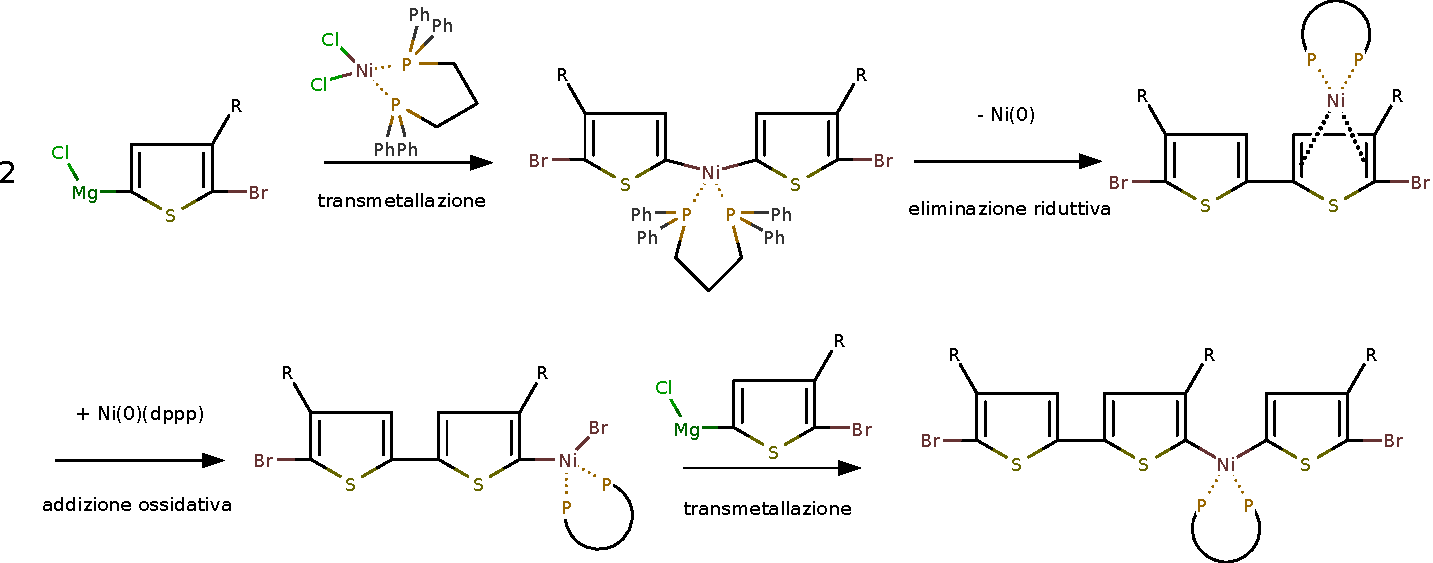
\includegraphics[width=1\textwidth]{img/syn-polimero-lunga.pdf}\end{figure}
\end{frame}
%X--%X--%X--%X--%X--%X--%X--%X--%X--%X--%X--%X--%X--%X--%X--%X--%X--%X--%X--%X--%X--%X--%X--%X--%X--%X--%X--%X--%X--%X--%X--
%X--%X--%X--%X--%X--%X--%X--%X--%X--%X--%X--%X--%X--%X--%X--%X--%X--%X--%X--%X--%X--%X--%X--%X--%X--%X--%X--%X--%X--%X--%X--
\subsection{Regioregolarità}
\begin{frame}% ============== regioregolarità ============== 
\frametitle{La regioregolarità}
\begin{tabular}{cc}
\multirow{3}{*}{
\onslide<2->{\includegraphics[width=.42\textwidth]{img/syn-metallazione.pdf}}
}&

\tallcell{regioregolare \\

\includegraphics[width=0.5\textwidth]{img/regioregolare2.pdf}}
\\
& \\
&

\tallcell{regio\textbf{ir}regolare\\

\includegraphics[width=0.5\textwidth]{img/regioirregolare2.pdf}}
\\
\end{tabular}

\vfill

\onslide<3->{{\hfill \textbf{Regioregolare} $\Rightarrow$ più lunghezza di \textbf{coniugazione} \hfill}

{\hfill$\Rightarrow$ migliore assorbimento (per una cella solare), \hfill}

{\hfill migliore conduzione (da una migliore aggregazione).\hfill} }
\end{frame}
%X--%X--%X--%X--%X--%X--%X--%X--%X--%X--%X--%X--%X--%X--%X--%X--%X--%X--%X--%X--%X--%X--%X--%X--%X--%X--%X--%X--%X--%X--%X--
%X--%X--%X--%X--%X--%X--%X--%X--%X--%X--%X--%X--%X--%X--%X--%X--%X--%X--%X--%X--%X--%X--%X--%X--%X--%X--%X--%X--%X--%X--%X--
\subsection{NMR}
\begin{frame}% ============== valutare regioregolarità ============== 
\frametitle{Come verifico la regioregolarità?}
Il chemical shift degli idrogeni sul tiofene risente dell'intorno.
\vfill
Un solo picco stretto per idrogeno $\Rightarrow$ \textbf{regioregolare}.
\vfill
\begin{figure}\centering \includegraphics[trim=0 0 348 0cm,clip,width=0.4\textwidth]{img/ig2-15-nmr-h.pdf}
\begin{minipage}{0.15\textwidth}\vspace{-100pt}
\includegraphics[width=1\textwidth]{img/polimero-idrogeni.pdf}
\end{minipage}
\includegraphics[trim=465 0 0 0cm,clip,width=0.3\textwidth]{img/ig2-15-nmr-h.pdf}\end{figure}
\end{frame}
%X--%X--%X--%X--%X--%X--%X--%X--%X--%X--%X--%X--%X--%X--%X--%X--%X--%X--%X--%X--%X--%X--%X--%X--%X--%X--%X--%X--%X--%X--%X--
%X--%X--%X--%X--%X--%X--%X--%X--%X--%X--%X--%X--%X--%X--%X--%X--%X--%X--%X--%X--%X--%X--%X--%X--%X--%X--%X--%X--%X--%X--%X--
\subsection{Massa}
\begin{frame}% ============== peso controllato ============== 
\frametitle{Quanto risulta lungo?}
La polimerizzazione che usiamo è quasi-vivente: permette il \textbf{controllo del grado di polimerizzazione} variando la quantità di catalizzatore e il tempo di polimerizzazione.
\vfill
Si ottiene \textbf{bassa polidispersità}.
\vfill
{\hfill
\begin{minipage}{.5\textwidth}\centering
\begin{figure}\centering 
\includegraphics[width=0.4\textwidth]{img/polidisperso.png}\\{\small polimero con alta polidispersità}
\end{figure}\end{minipage}\hfill
\begin{minipage}{.5\textwidth}\centering
\begin{figure}\centering 
\includegraphics[width=0.4\textwidth]{img/nonpolidisperso.png}\\{\small polimero con bassa polidispersità}
\end{figure}\end{minipage}\hfill}
\end{frame}
%X--%X--%X--%X--%X--%X--%X--%X--%X--%X--%X--%X--%X--%X--%X--%X--%X--%X--%X--%X--%X--%X--%X--%X--%X--%X--%X--%X--%X--%X--%X--
%X--%X--%X--%X--%X--%X--%X--%X--%X--%X--%X--%X--%X--%X--%X--%X--%X--%X--%X--%X--%X--%X--%X--%X--%X--%X--%X--%X--%X--%X--%X--
\subsection{SEC}
\begin{frame}% ============== sec ============== 
\frametitle{Come verifico la lunghezza?}
Cromatografia di esclusione molecolare (SEC) con riferimento di polistirene.
\vfill
\begin{columns}
\column{0.7\textwidth}
\begin{tabular}{c|c|c|c}
\toprule
\tallcell{{\footnotesize Metodo} \\{\footnotesize polimerizzazione}} & {\footnotesize Polimero} & \tallcell{{\footnotesize Unità} \\{\footnotesize ripetitive}} & {\footnotesize Polidispersità}\\\cmidrule{1-4}
Senza LiCl & P1  & 20  & 1.29 \\
\onslide<3->{Con LiCl}&\onslide<3->{P2} &\onslide<3->{80} & \onslide<3->{1.36} \\
\onslide<3->{Con LiCl}& \onslide<3->{ P2S} &  \onslide<3->{60} & \onslide<3->{1.32} \\
\bottomrule
\end{tabular} 

\column{0.3\textwidth}
\onslide<2->{Il primo polimero ha bassa massa, l'\textbf{aggiunta di LiCl migliora la polimerizzazione}.}

\end{columns}
\vfill

\onslide<3->{In ogni caso \textbf{polidispersità bassa}.}
\vfill
\onslide<3->{UV-vis conferma P1 molto corto, lo utilizziamo per \textbf{studi NMR-2D}.}
\end{frame}
%X--%X--%X--%X--%X--%X--%X--%X--%X--%X--%X--%X--%X--%X--%X--%X--%X--%X--%X--%X--%X--%X--%X--%X--%X--%X--%X--%X--%X--%X--%X--
%X--%X--%X--%X--%X--%X--%X--%X--%X--%X--%X--%X--%X--%X--%X--%X--%X--%X--%X--%X--%X--%X--%X--%X--%X--%X--%X--%X--%X--%X--%X--
\subsection{MALDI}
\begin{frame}% ============== maldi ============== 
\frametitle{Come si interrompono le catene?}

Spegnere la polimerizzazione con HCl$_{(acq)}$ dovrebbe eliminare il catalizzatore e inserire H, \textbf{risultato atteso: catene H/Br} terminate.
\vfill

\begin{figure}\centering 
\includegraphics[width=0.7\textwidth]{img/syn-quenching.pdf}
\end{figure}

\vfill
\pause
L'analisi di massa MALDI-TOF mostra varie terminazioni, purtroppo: \\ Br/H, Br/Br, Br/I, Br/OH, H/OH, Br/NiCl.
\end{frame}
%X--%X--%X--%X--%X--%X--%X--%X--%X--%X--%X--%X--%X--%X--%X--%X--%X--%X--%X--%X--%X--%X--%X--%X--%X--%X--%X--%X--%X--%X--%X--
%X--%X--%X--%X--%X--%X--%X--%X--%X--%X--%X--%X--%X--%X--%X--%X--%X--%X--%X--%X--%X--%X--%X--%X--%X--%X--%X--%X--%X--%X--%X--
\subsection{SEC-MALDI}
\begin{frame}% ============== sec-maldi ============== 
\frametitle{SEC -- MALDI}
\begin{figure}
  \includegraphics[width=0.9\textwidth]{img/ig2-8-sec-maldi2.png}
\end{figure}
\end{frame}
%X--%X--%X--%X--%X--%X--%X--%X--%X--%X--%X--%X--%X--%X--%X--%X--%X--%X--%X--%X--%X--%X--%X--%X--%X--%X--%X--%X--%X--%X--%X--
%X--%X--%X--%X--%X--%X--%X--%X--%X--%X--%X--%X--%X--%X--%X--%X--%X--%X--%X--%X--%X--%X--%X--%X--%X--%X--%X--%X--%X--%X--%X--
\section{Lo studio dell'aggregazione}
\subsection{UV-vis}
\begin{frame}% ============== cattivo solvente uvvis ============== 
\frametitle{Come si aggrega questo polimero?}
\pause
{\small\begin{tabular}{r|c}
Soluzioni di polimero in cloroformio o tetraidrofurano (\textbf{buoni solventi}) & +  \\
metanolo o acetonitrile (\textbf{cattivi solventi}) & = \\\cmidrule{1-2}
\multicolumn{1}{r}{\textbf{aggregazione}} & \\ 
\end{tabular}}
\pause

\begin{columns}
\column{0.52\linewidth} 
\begin{figure}\centering 
\includegraphics[width=1\textwidth]{img/ig2-8-vis-chcl3-meoh-freccia.jpg}
\end{figure}

\column{0.48\linewidth}

\begin{figure}
\begin{tikzpicture}
\begin{axis}[axis x line=bottom,axis y line=none,enlarge x limits=false,enlarge y limits=false,width=1\textwidth,height=4cm,xlabel=Lunghezza d'onda (nm),xmin=300,xmax=650,ymax=1.05,no markers]
\addplot[line width=1pt] table[y expr=\thisrowno{1}/1.04169] {img/ig2-15-uvvis-chcl3.txt};
\addplot[color=red,line width=1pt] table[y expr=\thisrowno{1}/1.8789] {img/ig2-15-uvvis-thf-55-ch3cn-45.txt};
\addplot[color=blue,line width=1pt] table[y expr=(\thisrowno{1}-0.15)/0.219712] {img/ig2-15-uvvis-cast-ch2cl2.txt};
\node[coordinate,pin=left:{\footnotesize CHCl$_3$}] at (axis cs:430,0.95304) {};
\node[coordinate,pin=right:{\footnotesize\color{red} THF-CH$_3$CN}] at (axis cs:320,0.17767) {};
\node[coordinate,pin=right:{\footnotesize\color{blue} solido}] at (axis cs:520,0.81902) {};
\end{axis}
\end{tikzpicture} 
\end{figure}
\end{columns}
\vfill  \pause

Si osserva un \textbf{red shift} degli assorbimenti,\\ causa intramolecolare: l'aumento della \textbf{lunghezza di coniugazione} \\e/o causa intermolecolare: l'\textbf{interazione tra catene parallele}.
\end{frame}
%X--%X--%X--%X--%X--%X--%X--%X--%X--%X--%X--%X--%X--%X--%X--%X--%X--%X--%X--%X--%X--%X--%X--%X--%X--%X--%X--%X--%X--%X--%X--
%X--%X--%X--%X--%X--%X--%X--%X--%X--%X--%X--%X--%X--%X--%X--%X--%X--%X--%X--%X--%X--%X--%X--%X--%X--%X--%X--%X--%X--%X--%X--
\subsection{PL}
\begin{frame}% ============== ee ============== 
\frametitle{Variando l'eccesso enantiomerico}
\begin{columns}
\column{0.45\linewidth}
Sintetizzati polimeri con diversa \textbf{stereo}regolarità utilizzando monomeri \textbf{più o meno enantiopuri}.
\bigskip\bigskip

\onslide<2->{Diversa fotoluminescenza aggiungendo cattivo solvente.}
\column{0.55\linewidth}
\centering
\onslide<2->{fotoluminescenza \\
\begin{figure}
\begin{tikzpicture}
\begin{axis}[axis x line=bottom,yticklabels={,,},axis y line=none,enlarge x limits=false,enlarge y limits=false,width=1\textwidth,height=7cm,xlabel=Lunghezza d'onda (nm),xmin=500,xmax=750,no markers,legend style={at={(1,1.1)},anchor=north east,font=\footnotesize},legend entries={enantiopuro,,,,enant. arricchito}]
\addplot[color=magenta,line width=1pt] table[y expr=\thisrowno{1}/10000] {img/ig2-8-pl-5480-chcl3.txt};
\addplot[color=magenta,line width=1pt] table[y expr=\thisrowno{1}/10000] {img/ig2-8-pl-137-chcl3-75-meoh-25.txt};
\addplot[color=magenta,line width=1pt] table[y expr=\thisrowno{1}/10000] {img/ig2-8-pl-137-chcl3-50-meoh-50.txt};
\addplot[color=magenta,line width=1pt] table[y expr=\thisrowno{1}/10000] {img/ig2-8-pl-137-chcl3-30-meoh-70.txt};
\addplot[color=green,line width=1pt] table[y expr=\thisrowno{1}/10000] {img/ig2-15-pl-5480-chcl3.txt};
\addplot[color=green,line width=1pt] table[y expr=\thisrowno{1}/10000] {img/ig2-15-pl-137-chcl3-75-meoh-25.txt};
\addplot[color=green,line width=1pt] table[y expr=\thisrowno{1}/10000] {img/ig2-15-pl-137-chcl3-50-meoh-50.txt};
\addplot[color=green,line width=1pt] table[y expr=\thisrowno{1}/10000] {img/ig2-15-pl-137-chcl3-30-meoh-70.txt};
\node[coordinate,pin=right:{\footnotesize\color{magenta} 0\% MeOH}] at (axis cs:600,1.19) {};
\node[coordinate,pin=right:{\footnotesize\color{magenta} 25\% MeOH}] at (axis cs:608,0.9) {};
\node[coordinate,pin=above:{\footnotesize\color{magenta} 50\% MeOH}] at (axis cs:630,0.12) {};
\node[coordinate,pin=above:{\footnotesize\color{magenta} 70\% MeOH}] at (axis cs:700,0.048) {};
\node[coordinate,pin=right:{\footnotesize\color{green} 0\% MeOH}] at (axis cs:622,1.04) {};
\node[coordinate,pin=right:{\footnotesize\color{green} 25\% MeOH}] at (axis cs:627,0.75) {};
\node[coordinate,pin=above:{\footnotesize\color{green} 50\% MeOH}] at (axis cs:591,0.6) {};
\node[coordinate,pin=above:{\footnotesize\color{green} 70\% MeOH}] at (axis cs:550,0.15) {};
\end{axis}
\end{tikzpicture}  
\end{figure}}
\end{columns}
\end{frame}
%X--%X--%X--%X--%X--%X--%X--%X--%X--%X--%X--%X--%X--%X--%X--%X--%X--%X--%X--%X--%X--%X--%X--%X--%X--%X--%X--%X--%X--%X--%X--
%X--%X--%X--%X--%X--%X--%X--%X--%X--%X--%X--%X--%X--%X--%X--%X--%X--%X--%X--%X--%X--%X--%X--%X--%X--%X--%X--%X--%X--%X--%X--
\subsection{CD}
\begin{frame}% ============== CD ============== 
\frametitle{Osservando il dicroismo circolare}
In soluzione di buon solvente nessun dicroismo circolare.
\vfill \pause
\begin{columns}
\column{0.3\textwidth}
Aggiungendo \textbf{cattivo solvente} e in stato solido ho un \textbf{picco bisegnato}.
\bigskip\bigskip

Il dicroismo circolare \textbf{rivela la formazione di aggregati}, prima dell'UV-vis.
\column{0.7\textwidth}
\begin{figure}
\begin{tikzpicture}
\begin{axis}[axis x line=bottom,axis y line=right,enlarge x limits=false,enlarge y limits=true,width=1\textwidth,height=6cm,xlabel=Lunghezza d'onda (nm),ylabel=Dicroismo circolare molare $\Delta\epsilon$,xmin=350,no markers]
\addplot[line width=1pt] table[y expr=\thisrowno{1}*0.403] {img/ig2-8-cd-137-chcl3-70-meoh-30-10min.txt};
\addplot[color=red,line width=1pt] table[y expr=\thisrowno{1}*0.403] {img/ig2-8-cd-137-chcl3-60-meoh-40.txt};
\addplot[color=green,line width=1pt] table[y expr=\thisrowno{1}*0.403] {img/ig2-8-cd-137-chcl3-50-meoh-50.txt};
\addplot[color=blue,line width=1pt] table[y expr=\thisrowno{1}*0.403] {img/ig2-8-cd-137-chcl3-40-meoh-60.txt};
\addplot[color=orange,line width=1pt] table[y expr=\thisrowno{1}*0.403] {img/ig2-8-cd-137-chcl3-30-meoh-70.txt};
\node[coordinate,pin=above:{\footnotesize 30\% MeOH}] at (axis cs:405,-0.959) {};
\node[coordinate,pin=below:{\footnotesize\color{red} 40\% MeOH}] at (axis cs:522,1.66) {};
\node[coordinate,pin=left:{\footnotesize\color{green} 50\% MeOH}] at (axis cs:470,2.42) {};
\node[coordinate,pin=right:{\footnotesize\color{blue} 60\% MeOH}] at (axis cs:513,3.58) {};
\node[coordinate,pin=right:{\footnotesize\color{orange} 70\% MeOH}] at (axis cs:510,4.69) {};
\end{axis}
\end{tikzpicture} 
\end{figure}
\end{columns}
\end{frame}
%X--%X--%X--%X--%X--%X--%X--%X--%X--%X--%X--%X--%X--%X--%X--%X--%X--%X--%X--%X--%X--%X--%X--%X--%X--%X--%X--%X--%X--%X--%X--
%X--%X--%X--%X--%X--%X--%X--%X--%X--%X--%X--%X--%X--%X--%X--%X--%X--%X--%X--%X--%X--%X--%X--%X--%X--%X--%X--%X--%X--%X--%X--
\subsection{Origine CD}
\begin{frame}% ============== origine ============== 
\frametitle{Qual è l'origine del dicroismo circolare?}
Eliche di \textbf{singola catena}?
\vfill
Origine intermolecolare da \textbf{interazione di più catene}?
\vfill
\begin{figure}\centering\includegraphics[width=1\textwidth]{img/conformazioni2.png}\end{figure}
\end{frame}
%X--%X--%X--%X--%X--%X--%X--%X--%X--%X--%X--%X--%X--%X--%X--%X--%X--%X--%X--%X--%X--%X--%X--%X--%X--%X--%X--%X--%X--%X--%X--
%X--%X--%X--%X--%X--%X--%X--%X--%X--%X--%X--%X--%X--%X--%X--%X--%X--%X--%X--%X--%X--%X--%X--%X--%X--%X--%X--%X--%X--%X--%X--
\subsection{Concentrazione}
\begin{frame}% ============== CD concentrazione ============== 
\frametitle{Variando la concentrazione}
\begin{columns}
\column{0.5\linewidth} 
Un processo \textbf{intermolecolare} deve mostrare \textbf{dipendenza dalla concentrazione}.
\column{0.5\linewidth}
\begin{figure}
\vspace{-20pt}
\centering\includegraphics[width=1\textwidth]{img/conformazioni-piani2.png}\end{figure}
\end{columns}
\vspace{-20pt}\pause
\begin{columns}
\column{0.4\linewidth} 
Esperimento a concentrazione variabile in \\ 50~\% THF -- 50~\% acetonitrile:

\bigskip\bigskip
Fattore di dissimmetria: $g = \frac{\Delta\epsilon}{\epsilon}$ dunque indipendente dalla concentrazione.
\column{0.6\linewidth}
\begin{figure}
\begin{tikzpicture}
\begin{axis}[axis x line=bottom,axis y line=right,enlarge x limits=false,enlarge y limits=true,width=1\textwidth,height=6cm,xlabel=Lunghezza d'onda (nm),ylabel=Fattore di dissimmetria m$g$,xmin=300,xmax=570,legend pos=north west,no markers,legend style={font=\footnotesize}]
\addplot[line width=1pt] table[y expr=\thisrowno{1}*1000] {img/ig2-15-g-137-thf-50-ch3cn-50.txt};
\addlegendentry{\SI{137}{\mg\per\liter}};
\addplot[color=red,line width=1pt] table[y expr=\thisrowno{1}*1000] {img/ig2-15-g-274-thf-50-ch3cn-50.txt};
\addlegendentry{\SI{274}{\mg\per\liter}};
\addplot[color=green,line width=1pt] table[y expr=\thisrowno{1}*1000] {img/ig2-15-g-548-thf-50-ch3cn-50.txt};
\addlegendentry{\SI{548}{\mg\per\liter}};
\end{axis}
\end{tikzpicture}
\end{figure}
\end{columns}
\end{frame}
%X--%X--%X--%X--%X--%X--%X--%X--%X--%X--%X--%X--%X--%X--%X--%X--%X--%X--%X--%X--%X--%X--%X--%X--%X--%X--%X--%X--%X--%X--%X--
%X--%X--%X--%X--%X--%X--%X--%X--%X--%X--%X--%X--%X--%X--%X--%X--%X--%X--%X--%X--%X--%X--%X--%X--%X--%X--%X--%X--%X--%X--%X--
\subsection{XRD}
\begin{frame}% ============== XRD ============== 
\frametitle{Diffrazione a raggi X}
Da XRD e da SAXS, sia su solido bulk che su film sottile, si osserva \textbf{copresenza di domini cristallini e regioni amorfe}.

\vspace{-10pt}
\begin{columns}
\column{0.7\linewidth}
\begin{figure}
\begin{tikzpicture}
\begin{axis}[axis x line=bottom,axis y line=none,enlarge x limits=false,enlarge y limits=false,width=1\textwidth,height=4cm,yticklabels={,,},xlabel=Angolo $2\theta$,ylabel=Intensity (a.\ u.),xmin=2]
\addplot[line width=1pt] table {img/ig2-8-xrd-cast-ch2cl2-Perp_32_00001IP.txt};
\node[coordinate,pin=right:{\footnotesize interdigitazione (100)}] at (axis cs:4.98197,21807.2) {};
\node[coordinate,pin=above:{\footnotesize interd.(200)}] at (axis cs:10.1615,5223.51) {};
\node[coordinate,pin=above:{\footnotesize interd.(300)}] at (axis cs:15.2532,7580.33) {};
\node[coordinate,pin=right:{\footnotesize amorfo}] at (axis cs:21,9213.02) {};
\end{axis}
\end{tikzpicture}  
\end{figure}
\column{0.3\linewidth}
\begin{figure}\centering 
\includegraphics[width=1\textwidth]{img/lamella.pdf}
\end{figure}
\end{columns}

\bigskip
L'interpretazione del dicroismo circolare è ancora in corso, nuovi studi, ad esempio di NMR, sono in programma.
\end{frame}
%X--%X--%X--%X--%X--%X--%X--%X--%X--%X--%X--%X--%X--%X--%X--%X--%X--%X--%X--%X--%X--%X--%X--%X--%X--%X--%X--%X--%X--%X--%X--
%X--%X--%X--%X--%X--%X--%X--%X--%X--%X--%X--%X--%X--%X--%X--%X--%X--%X--%X--%X--%X--%X--%X--%X--%X--%X--%X--%X--%X--%X--%X--

\makeatletter
\setbeamertemplate{footline}{}
\makeatother

\section{I problemi affrontati nella tesi - 2}
\subsection{Blocchi}
\begin{frame}% ============== blocchi ============== 
\frametitle{Copolimero a blocchi}
{\hfill Dal politiofene è stato sintetizzato un polimero a blocchi \hfill}

{\hfill \textbf{{\color{red}politiofene} -- {\color{blue}polivinilpiridina}}. \hfill}
\begin{figure}\centering \includegraphics[width=1.15\textwidth]{img/blocchi-fullereni-colori.pdf}\vspace{-90pt}\end{figure}
\end{frame}

\makeatletter
\setbeamertemplate{footline}
{
  \leavevmode%
  \hbox{%
  \begin{beamercolorbox}[wd=.20\paperwidth,ht=2.25ex,dp=1ex,center]{section in head/foot}%
    \usebeamerfont{author in head/foot}Ilario Gelmetti
  \end{beamercolorbox}%
  \begin{beamercolorbox}[wd=.55\paperwidth,ht=2.25ex,dp=1ex,center]{section in head/foot}%
    \usebeamerfont{title in head/foot}\insertsection
  \hfill $>$ \hfill
    \usebeamerfont{title in head/foot}\insertsubsection
  \end{beamercolorbox}%
  \begin{beamercolorbox}[wd=.25\paperwidth,ht=2.25ex,dp=1ex,right]{section in head/foot}%
    \usebeamerfont{date in head/foot}\insertshortdate{}\hspace*{2em}
    \insertframenumber{} / \inserttotalframenumber\hspace*{2ex} 
  \end{beamercolorbox}}%
  \vskip0pt%
}
\makeatother
\logo{\includegraphics[width=0.1\paperwidth]{img/unipi-logo_con_testo-small.png}}
%X--%X--%X--%X--%X--%X--%X--%X--%X--%X--%X--%X--%X--%X--%X--%X--%X--%X--%X--%X--%X--%X--%X--%X--%X--%X--%X--%X--%X--%X--%X--
%X--%X--%X--%X--%X--%X--%X--%X--%X--%X--%X--%X--%X--%X--%X--%X--%X--%X--%X--%X--%X--%X--%X--%X--%X--%X--%X--%X--%X--%X--%X--
\subsection{Dispersione}
\begin{frame}% ============== blocchi perché ============== 
\frametitle{Perché utilizzare un polimero a blocchi?}

Si aggiunge un secondo blocco polimerico per:
\bigskip
\begin{enumerate}
\item \textbf{stabilizzare} la dispersione (i materiali immiscibili tendono a segregare eccessivamente, limitare la dimensione dei domini)
\end{enumerate}

\begin{columns}
\column{0.5\textwidth}
\begin{enumerate}
\setcounter{enumi}{1}
\item \textbf{controllare la morfologia} della dispersione (evitare la formazione di domini isolati)
\end{enumerate}
\column{0.47\textwidth}
\begin{figure}\centering \includegraphics[width=1\textwidth]{img/bhj4.pdf}\end{figure}
\end{columns}


\end{frame}
%X--%X--%X--%X--%X--%X--%X--%X--%X--%X--%X--%X--%X--%X--%X--%X--%X--%X--%X--%X--%X--%X--%X--%X--%X--%X--%X--%X--%X--%X--%X--
%X--%X--%X--%X--%X--%X--%X--%X--%X--%X--%X--%X--%X--%X--%X--%X--%X--%X--%X--%X--%X--%X--%X--%X--%X--%X--%X--%X--%X--%X--%X--
\subsection{Stabilizzazione}
\begin{frame}% ============== stabilizzare dispersione ============== 
\frametitle{1. Stabilizzare la dispersione}
Usiamo un polimero \textbf{anfifilico} a blocchi. 
\vfill

Il \textbf{politiofene si aggrega} per $\pi-\pi$ stacking, la \textbf{polivinilpiridina} è legata covalentemente al politiofene e \textbf{coordina i fullereni}.
\vfill
Questo permette una \textbf{nanosegregazione} ma impedisce lo smescolamento.
\vfill
\begin{figure}\centering \includegraphics[width=.7\textwidth]{img/blocchi_PCBM-testo.png}\end{figure}
\end{frame}
%X--%X--%X--%X--%X--%X--%X--%X--%X--%X--%X--%X--%X--%X--%X--%X--%X--%X--%X--%X--%X--%X--%X--%X--%X--%X--%X--%X--%X--%X--%X--
%X--%X--%X--%X--%X--%X--%X--%X--%X--%X--%X--%X--%X--%X--%X--%X--%X--%X--%X--%X--%X--%X--%X--%X--%X--%X--%X--%X--%X--%X--%X--
\subsection{Morfologia}
\begin{frame}% ============== controllare dispersione ============== 
\frametitle{2. Controllare la morfologia della dispersione}
\onslide<1->{Variando la lunghezza dei due blocchi e la quantità di fullerene si hanno \textbf{morfologie più o meno efficienti}.}
\vfill 
\onslide<2->{I domini isolati sono trappole per le cariche.}
\vfill 
\onslide<2->{\textbf{Necessario avere il controllo sul grado di polimerizzazione.}}
\vfill
\onslide<1->{\begin{figure}\centering \includegraphics[width=0.7\textwidth]{img/morfologia2.png}\end{figure}}
\vspace{-20pt}
{\tiny Topham, Parnell, Hiorns. Block copolymer strategies for solar cell technology. \textit{J. Polym. Sci. Part B} 2011; 49:1131–1156.}
\end{frame}
%X--%X--%X--%X--%X--%X--%X--%X--%X--%X--%X--%X--%X--%X--%X--%X--%X--%X--%X--%X--%X--%X--%X--%X--%X--%X--%X--%X--%X--%X--%X--
%X--%X--%X--%X--%X--%X--%X--%X--%X--%X--%X--%X--%X--%X--%X--%X--%X--%X--%X--%X--%X--%X--%X--%X--%X--%X--%X--%X--%X--%X--%X--
\section{La sintesi del secondo blocco}
\subsection{Aldeide}
\begin{frame}% ============== aldeide ============== 
\frametitle{Sintesi del macroiniziatore per il secondo blocco}
\begin{figure}\centering \includegraphics[width=1\textwidth]{img/syn-aldeide.pdf}
\end{figure}
\vfill

\begin{figure}\centering \includegraphics[width=0.8\textwidth]{img/syn-tipno-li.pdf}
\end{figure}
\end{frame}
%X--%X--%X--%X--%X--%X--%X--%X--%X--%X--%X--%X--%X--%X--%X--%X--%X--%X--%X--%X--%X--%X--%X--%X--%X--%X--%X--%X--%X--%X--%X--
%X--%X--%X--%X--%X--%X--%X--%X--%X--%X--%X--%X--%X--%X--%X--%X--%X--%X--%X--%X--%X--%X--%X--%X--%X--%X--%X--%X--%X--%X--%X--
\subsection{Polimerizzazione}
\begin{frame}% ============== P4VP ============== 
\frametitle{Polimerizzazione della vinilpiridina}
\begin{figure}\centering \includegraphics[width=1\textwidth]{img/syn-blocco.pdf}\end{figure}
\end{frame}
%X--%X--%X--%X--%X--%X--%X--%X--%X--%X--%X--%X--%X--%X--%X--%X--%X--%X--%X--%X--%X--%X--%X--%X--%X--%X--%X--%X--%X--%X--%X--
%X--%X--%X--%X--%X--%X--%X--%X--%X--%X--%X--%X--%X--%X--%X--%X--%X--%X--%X--%X--%X--%X--%X--%X--%X--%X--%X--%X--%X--%X--%X--
\subsection{NMR e CD}
\begin{frame}% ============== nmr e cd ============== 
\frametitle{Caratterizzazione preliminare}
$^1$H-NMR: il blocco di politiofene ha 5 volte più unità ripetitive del blocco di polivinilpiridina.
\vfill
Dicroismo circolare in cloroformio -- metanolo: il metanolo è un cattivo solvente per il politiofene ma buon solvente per la polivinilpiridina.

In cloroformio-metanolo l'\textbf{omopolimero} si aggrega dal \textbf{30\% di metanolo} mentre il \textbf{polimero a blocchi} si aggrega dal \textbf{40\% di metanolo}. 
\end{frame}
%X--%X--%X--%X--%X--%X--%X--%X--%X--%X--%X--%X--%X--%X--%X--%X--%X--%X--%X--%X--%X--%X--%X--%X--%X--%X--%X--%X--%X--%X--%X--
%X--%X--%X--%X--%X--%X--%X--%X--%X--%X--%X--%X--%X--%X--%X--%X--%X--%X--%X--%X--%X--%X--%X--%X--%X--%X--%X--%X--%X--%X--%X--
\section{Il test in cella solare}
\subsection{$V_{oc}$}
\begin{frame}% ============== cella ============== 
\frametitle{Test del politiofene omopolimero in cella solare}

\begin{figure}\centering \includegraphics[width=0.4\textwidth]{img/polimero_PCBM-colorato.pdf}\end{figure}
\pause 

\begin{table}
\centering
\begin{tabular}{c|c|c|c|c}
\toprule
\tallcell{Polimero \\donore} & {$V_{oc}$ (\SI{}{\mV})} & {$J_{sc}$ (\SI{}{\mA\per\square\cm})} & {FF (\%)}& {$\eta$ (\%)}\\\cmidrule{1-5}
P3HT &0,567$\pm$0,007&\onslide<3->{-10,7$\pm$0,6}&\onslide<3->{50$\pm$20}&\onslide<3->{3$\pm$1} \\
P2S & 0,67$\pm$0,05&\onslide<3->{-3,2$\pm$0,5}&\onslide<3->{31$\pm$3}&\onslide<3->{0,7$\pm$0,1}  \\
\bottomrule
\end{tabular}
\end{table}
\vfill

In cella solare il nostro polimero ha dato \textbf{voltaggio $V_{oc}$ maggiore} del materiale di riferimento (poli(3-esiltiofene):PCBM).

\end{frame}
%X--%X--%X--%X--%X--%X--%X--%X--%X--%X--%X--%X--%X--%X--%X--%X--%X--%X--%X--%X--%X--%X--%X--%X--%X--%X--%X--%X--%X--%X--%X--
%X--%X--%X--%X--%X--%X--%X--%X--%X--%X--%X--%X--%X--%X--%X--%X--%X--%X--%X--%X--%X--%X--%X--%X--%X--%X--%X--%X--%X--%X--%X--
\section{Conclusioni}
\subsection{Conclusioni}
\begin{frame}% ============== conclusioni ============== 
\frametitle{Conclusioni}
\begin{itemize}
\item Abbiamo portato un contributo allo studio dell'origine dell'attività ottica nei politiofeni chirali.
\item Abbiamo realizzato una cella solare mostrando l'influenza delle caratteristiche del materiale scelto sulle proprietà elettriche.
\item Abbiamo sintetizzato un copolimero a blocchi adatto ad essere impiegato in celle solari.
\item Abbiamo introdotto la spettroscopia di dicroismo circolare come metodo di indagine di stati aggregati disordinati.
\end{itemize}
\pause
\vfill
\begin{center}
\Huge \textbf{Grazie per l'attenzione.}

\includegraphics[width=0.12\textwidth]{img/cc-by-sa.pdf} - Source code available - \texttt{ilario.gelmetti@sns.it, iochesonome@gmail.com}


\end{center}
\end{frame}
%X--%X--%X--%X--%X--%X--%X--%X--%X--%X--%X--%X--%X--%X--%X--%X--%X--%X--%X--%X--%X--%X--%X--%X--%X--%X--%X--%X--%X--%X--%X--
%X--%X--%X--%X--%X--%X--%X--%X--%X--%X--%X--%X--%X--%X--%X--%X--%X--%X--%X--%X--%X--%X--%X--%X--%X--%X--%X--%X--%X--%X--%X--
\end{document}
